\documentclass[12pt,draft]{thesis-umich}

%\input{listingsConfig}
\usepackage{titletoc}
\dottedcontents{subsection}[6.7em]{}{3.2em}{1pc}
\dottedcontents{subsubsection}[8.7em]{}{3.2em}{1pc}
\usepackage{hyperref}
\usepackage{mathtools}
\usepackage{appendix}
\usepackage{titletoc}
\usepackage{amsmath}
\usepackage[format=hang,font={bf}]{caption}
\usepackage{bm}
\usepackage{multirow}
\usepackage{ifdraft}
\usepackage{todonotes}
\usepackage{flexisym}
\usepackage{breqn}
\usepackage{tikz}
\usetikzlibrary{shapes,arrows}

% Set up flowchart stuff
\tikzstyle{startstop} = [rectangle, rounded corners, minimum width=3cm, minimum height=1cm,text centered, draw=black, fill=red!30]
\tikzstyle{io} = [trapezium, trapezium left angle=70, trapezium right angle=110, minimum width=3cm, minimum height=1cm, text centered, draw=black, fill=blue!30]
\tikzstyle{process} = [rectangle, minimum width=3cm, minimum height=1cm, text centered, text width=3cm, draw=black, fill=orange!30]
\tikzstyle{decision} = [diamond, minimum width=3cm, minimum height=1cm, text centered, draw=black, fill=green!30]
\tikzstyle{arrow} = [thick,->,>=stealth]

% Set up refs
\hypersetup{
    colorlinks,
    citecolor=red,
    filecolor=black,
    linkcolor=black,
    urlcolor=black
}
\setcounter{tocdepth}{4}
\setcounter{secnumdepth}{4}

\newcommand*{\bfrac}[2]{\genfrac{}{}{0pt}{}{#1}{#2}}
\dottedcontents{subsection}[6.0em]{}{2.8em}{1pc}
\dottedcontents{subsubsection}[9.0em]{}{3.5em}{1pc}
% \renewcommand{\thefigure}{\textbf{Figure \arabic{section}}}
% \renewcommand \thesection{\Roman{section}.}rand

\begin{document}

%\titlepage

\pagenumbering{arabic}

\chapter{Introduction}
\begin{itemize}
    \item Importance of predicting flux distributions (safety, economics)
    \item Historical reactor analysis methods
    \item shift toward direct whole-core transport
    \item Monte Carlo \& Deterministic
\end{itemize}

\section{Motivation}

\begin{itemize}
    \item Planar Synthesis Methods
    \item Need for Speed
    \item Axial Heterogeneities
\end{itemize}

\section{Previous Work in 2D/1D}

\begin{itemize}
    \item Introduce rod cusping as most significant heterogeneity
    \item Briefly discuss prior methods used to address rod cusping
    \item Mention general limitations of these methods to motivate new ones
\end{itemize}

\section{Dissertation Overview}

\begin{itemize}
    \item Introduction to transport theory, including standard/relevant approximations to the equation \& numerical methods to solve it
    \item Description of the 2D/1D Method.  Introduce MPACT at this point?
    \item History of prior rod cusping methods, both nodal and whole-core transport
    \item Description of methods I've developed
    \item Results \& Analysis
    \item Conclusions \& Future Work
\end{itemize}
\ifdraft{\todo{punctuate equations correctly and consistently}}{}
\todo{Format equation references appropriately}

\chapter{Neutron Transport Methodology}\label{chap:transport}
\section{Boltzmann Equation}

The Boltzmann equation for neutron transport is shown below: \hl{Some kind of background or derivation of this?}

\begin{gather}\label{e:boltzmann}
\frac{1}{v} \frac{\partial \psi}{\partial t} + \bm \Omega \cdot \bm \nabla \psi + \Sigma_t\left(x,E,t\right)\psi\left(x,E,\bm \Omega,t\right) = \intop_{4\pi} \Sigma_s\left(x,E' \rightarrow E, \bm \Omega' \rightarrow \bm \Omega, t\right) \psi\left(x,E',\bm \Omega',t\right) d\bm \Omega' + \nonumber\\
\frac{\chi\left(E\right)}{4\pi} \intop \nu \Sigma_f\left(x,E,t\right) \psi\left(x,E,\bm \Omega,t\right) dE + Q\left(x,E,\bm \Omega,t\right)
\end{gather}

For many problems, the time dependence of the Boltzmann equation can be neglected.  Doing do eliminates the first term of the equation above.  In order to ensure neutron balance, this equation is normally formulated as an eigenvalue problem.  The eigenvalue $\lambda = \frac{1}{k}$ allows the two sides of the equation to balance.  The cross-sections can then be adjusted until $\lambda = 1$ is achieved, which is the only meaningful solution for steady-state problems.  The eigenvalue form of the Boltzmann equation is shown below:

\begin{gather}\label{e:ssboltzmann}
\bm \Omega \cdot \bm \nabla \psi + \Sigma_t\left(x,E\right)\psi\left(x,E,\bm \Omega\right) = \intop_{4\pi} \Sigma_s\left(x,E' \rightarrow E, \bm \Omega' \rightarrow \bm \Omega\right) \psi\left(x,E',\bm \Omega'\right) d\bm \Omega' + \nonumber\\
\frac{1}{k}\frac{\chi\left(E\right)}{4\pi} \intop \nu \Sigma_f\left(x,E\right) \psi\left(x,E,\bm \Omega\right) dE + Q\left(x,E,\bm \Omega\right)
\end{gather}

\subsection{Multi-group Approximation}

One important approximation that is commonly made to the transport equation is the multi-group approximation.  To make this approximation, an appropriate energy range for the problem of interest is selected.  This energy range is divided up into $N$ energy groups, with each group going from $E_g$ up to $E_{g-1}$.  For light-water reactor problems, it is common to select 0 eV for $E_N$ and 20 MeV for $E_0$.  Once an appropriate group structure has been selected, equation \ref{e:ssboltzmann} (\hl{or} \ref{e:boltzmann}) is operated on by 

\begin{equation}
\frac{1}{E_{n-1} - E_n}\intop_{E_n}^{E_{n-1}}\left(\cdot\right)dE
\end{equation}

for each energy group, giving the following result:

\begin{gather}
\bm \Omega \cdot \bm \nabla \psi_g + \Sigma_{t,g}\left(x\right)\psi_g\left(x,\bm \Omega\right) = \intop_{4\pi} \Sigma_{s,g'\rightarrow}\left(x,\bm \Omega' \rightarrow \bm \Omega\right) \psi_{g'}\left(x,\bm \Omega'\right) d\bm \Omega' + \nonumber\\
\frac{1}{k}\frac{\chi_g}{4\pi} \sum_{g'=1}^{G} \nu \Sigma_{f,g'}\left(x,t\right) \psi_{g'}\left(x,\bm \Omega\right) + Q_g\left(x,\bm \Omega\right)\label{e:multigroupboltzmann}
\end{gather}

In equation \ref{e:multigroupboltzmann}, $\psi_g$ denotes the average angular flux for group $g$, defined as

\begin{equation}\label{e:multigroupangflux}
\psi_g\left(x,\bm \Omega\right)=\frac{1}{E_{n-1}-E_n} \intop_{E_n}^{E_{n-1}} \psi\left(x,E,\bm\Omega\right) dE
\end{equation}

The quantities that we want to preserve through the use of the multi-group approximation are the total reaction rates.  To do this, we must define the multi-group cross-sections as follows:

\begin{equation}\label{e:multigroupXS}
\Sigma_x,g \psi_g = \frac{1}{E_{n-1}-E_n} \intop_{E_n}^{E_{n-1}} \psi\left(E\right) \Sigma_x\left(E\right) dE \Rightarrow \Sigma_x,g = \frac{\intop_{E_n}^{E_{n-1}} \psi\left(E\right) \Sigma_x\left(E\right) dE}{\intop_{E_n}^{E_{n-1}} \psi\left(x,E,\bm\Omega\right) dE}
\end{equation}

This definition of the multi-group flux and multi-group cross-sections guarantees that the total reaction rates in each group will be preserved.

\hl{Talk about the dependence of the XS on the solution?}

\subsection{Spherical Harmonics Approximation}

One of the biggest challenges to solving the transport equation is angle dependence of the scattering cross-sections and angular flux.  To simplify the equation while preserving accuracy of the transport equation, the spherical harmonics approximation is applied to the scattering cross-sections.  This approximation assumes that the angle dependence of the scattering cross-sections can be represented as a series of Legendre polynomials with corresponding coefficients, shown in equation \hl{need an equation}:

\begin{equation}\label{e:sphericalHarmonicsXSExpansion}
\end{equation}

All Legendre polynomials are orthonormal, meaning that each $n$-th polynomial has the following properties:

\begin{subequations}
\begin{equation}
\intop_{-1}^1 P_n\left(x\right) dx =
\end{equation}
\begin{equation}
\intop_{-1}^1 P_n\left(x\right) P_m\left(x\right) dx = \delta_{n,m} = \begin{cases} 1, & n = m \\
0, & n \neq m
\end{cases}
\end{equation}
\end{subequations}

Before proceeding, an important simplification must be made to the scattering source.  The differential scattering cross-section depends on the term $\bm \Omega' \cdot \bm \Omega$, the scalar product between the incoming and outgoing directions.  However, this product is simply the cosine of the angle between the two directions $\mu$.  Using this fact, we can rewrite the scattering source in equation \ref{e:ssboltzmann} as follows:

\begin{equation}
\intop_{4\pi} \Sigma_s\left(x,E' \rightarrow E,\bm \Omega' \rightarrow \bm \Omega\right)\psi\left(x,E',\bm\Omega'\right)d\bm\Omega' = \intop_0^{2\pi} \intop_{-1}^1 \Sigma_s\left(x,E' \rightarrow E,\mu'\right) \psi\left(x,E',\bm\Omega'\right) d\mu' d\gamma'
\end{equation}

\hl{Look at Larsen's notes to remember the exact mathematical details of this}

\subsection{Diffusion Approximation}

\hl{All over this, but need to finish up the Pn stuff first}

\subsection{Transport Correction}

\hl{Not 100\% sure if this even needs to exist at all}

\section{Numerical Methods}

A wide variety of numerical methods exist to solve the transport equation, but all of them can be categorized in one of two ways: stochastic (Monte Carlo) or deterministic methods.  Monte Carlo methods use random numbers to directly sample probability distribution functions based on the material cross-sections.  These methods can produce highly accurate, detailed results and make no assumptions about the materials or geometry of the problem.  However, because of the random nature of the method, there is always some uncertainty in the answer.  For large problems, the number of particles that must be simulated to achieve acceptable levels of uncertainty is often \hl{need a better word here} too burdensome for practical calculations.

All the work discussed in the following sections makes use of deterministic methods.  There are many different deterministic methods, but only the ones relevant to this work will be discussed in the coming sections.

\subsection{Method of Characteristics}

One method that is commonly used to solve the transport equation is the Method of Characteristics (MOC).  This method allows the transport equation to be solved along a characteristic direction without any approximations, making it useful for complicated geometries, such as those found in nuclear reactors.  To derive this method, the right-hand side of equation \ref{e:ssboltzmann} is replaced by the variable $q$:

\begin{subequations}
\begin{equation}
\bm \Omega \cdot \bm \nabla \psi + \Sigma_t\left(x,E\right)\psi\left(x,E,\bm \Omega\right) = q\left(x,E.\bm \Omega\right)
\end{equation}
\begin{gather}\label{e:MOCqboltzmann}
q\left(x,E,\bm \Omega\right) = \intop_{4\pi} \Sigma_s\left(x,E' \rightarrow E, \bm \Omega' \rightarrow \bm \Omega\right) \psi\left(x,E',\bm \Omega'\right) d\bm \Omega' +\nonumber\\
\frac{1}{k}\frac{\chi\left(E\right)}{4\pi} \intop \nu \Sigma_f\left(x,E\right) \psi\left(x,E,\bm \Omega\right) dE + Q\left(x,E,\bm \Omega\right)
\end{gather}
\end{subequations}

Now the characteristic direction is introduced:

\begin{equation}
\bm r = \bm {r_0} + s \bm \Omega \Rightarrow \begin{cases} x\left(s\right) = x_0 + s\Omega_x \\ y\left(s\right) = y_0 + s\Omega_y \\ z\left(s\right) = z_0 + s\Omega_z\end{cases}
\end{equation}

Substituting this variable into equation \ref{e:MOCqboltzmann} gives the characteristic form of this equation:

\begin{subequations}
\begin{equation}
\frac{\partial \psi}{\partial s} + \Sigma_t\left(\bm r0_0 + s\bm\Omega,E\right)\psi\left(\bm r0_0 + s\bm\Omega,E,\bm \Omega\right) = q\left(\bm r0_0 + s\bm\Omega,E.\bm \Omega\right)
\end{equation}
\begin{gather}\label{e:characteristicboltzmann}
q\left(\bm r0_0 + s\bm\Omega,E,\bm \Omega\right) = \intop_{4\pi} \Sigma_s\left(\bm {r_0} + s \bm\Omega',E' \rightarrow E, \bm \Omega' \rightarrow \bm \Omega\right) \psi\left(\bm {r_0} + s\bm\Omega',E',\bm \Omega'\right) d\bm \Omega' +\nonumber\\
\frac{1}{k}\frac{\chi\left(E\right)}{4\pi} \intop \nu \Sigma_f\left(\bm r0_0 + s\bm\Omega,E\right) \psi\left(\bm {r_0} + s\bm\Omega,E,\bm \Omega\right) dE + Q\left(\bm {r_0} + s\bm\Omega,E,\bm \Omega\right)
\end{gather}
\end{subequations}

This equation is easily solved using an integrating factor

\begin{equation}
\exp{-\intop_0^s \Sigma_t\left(\bm {r_0} + s'\bm\Omega,E\right)ds'}
\end{equation}

giving the following solution:

\begin{gather}\label{e:MOCexact}
\psi\left(\bm {r_0} + s\bm\Omega,\bm\Omega,E\right) = \psi\left(\bm {r_0},\bm\Omega,E\right)\exp{\left(-\intop_0^s \Sigma_t\left(\bm {r_0} + s'\bm\Omega,E\right)ds'\right)} + \nonumber\\
\intop_0^s q\left(\bm {r_0} + s'\bm\Omega,\bm\Omega, E\right)\exp{\left(-\intop_0^s \Sigma_t\left(\bm {r_0} + s''\bm\Omega,E\right)ds''\right)}ds'
\end{gather}

Now if $\bm {r_0}$ is on the boundary of the region of interest, the incoming flux $\psi\left(\bm {r_0},\bm \Omega, E\right)$ is known.  This allows the angular flux to be calculated at any point $s$ to be calculated along the characteristic direction $\bm r$.

Up to this point, no approximations have been made in deriving the method of characteristics.  One approximation that is necessary to use MOC for practical problems is to assume some spatial shape for the source term $q$.  The simplest of these is the flat source approximation.  In this approximation, $q$ is assumed to be flat along $\bm r$.  This simplifies equation \ref{e:MOCexact} to the following:

\begin{gather}\label{e:MOCflatsource}
\psi\left(\bm {r_0} + s\bm\Omega,\bm\Omega,E\right) = \psi\left(\bm {r_0},\bm\Omega,E\right)\exp{\left(-\intop_0^s \Sigma_t\left(\bm {r_0} + s'\bm\Omega,E\right)ds'\right)} + ...
\end{gather}
% Derive it!
% Things to talk about:
%   Flat/linear sources

\subsection{Source Iteration}

Using MOC, fixed source transport problems can be solved.  However, in realistic calculations it is rare that the scattering or fission sources are known.  In order to solve the transport equation for problems with an unknown source distribution, the equation can be re-formulated as follows:

\hl{Insert source iteration form of the equation}

Now making some initial guess for \hl{$\phi^-1$} allows us to solve for \hl{$\phi^0$}.  This process can be repeated for all \hl{$\phi^n$} using the previous iterate \hl{variable$\phi^{n-1}$}.  This method is known as Source Iteration (SI).

Source iteration also has a convenient physical interpretation.  Selecting zero as the initial guess means that the first iterate \hl{$\phi^0$} is simply equal to the sum of sources of new neutrons.  Plugging the expression for \hl{$\phi^0$} into the equation for \hl{$\phi^1$}, we find that the \hl{$\phi^1$} is 

\hl{make sure to talk about how ridiculously slowly it can converge.  Find some references for the math if possible}

\subsection{Coarse-Mesh Finite Difference}

The source iteration method provides a convenient way of solving transport problems that guarantees a positive, correct solution.  However, because the source iteration can take hundreds of iterations to converge for typical reactor problems, it is important to accelerate the convergence.  The most common way of doing this is the Coarse-Mesh Finite Difference (CMFD) method.  This method involves solving a diffusion problem on a coarse grid to get the average magnitude of the flux in each coarse cell.  This is then used to scale the flux solution on the fine mesh cells.  In order to ensure consistency between the transport solution and the lower order diffusion solution, coupling coefficients are calculated on the boundaries of the coarse mesh cells to correct the leakage between the cells.

To derive this method, we begin with equation \hl{diffusion equation} and apply the multigroup approximation:
\hl{multi-group diffusion equation}

\begin{equation}
\end{equation}

Integrating this equation over some volume $V$ and dividing by the total volume creates and equation for the average scalar flux $\overline{\phi}$ in that cell.
\hl{discretized equation}

\begin{equation}
\end{equation}

The boundary conditions for each cell are the currents at the interface between two cells:
\hl{boundary condition equation}

\begin{equation}
\end{equation}

This equation can be determined for each cell in the problem to set up a linear system.  This system can then be solved using one of a variety of standard linear solvers.

Because the currents in the matrix are calculated from the diffusion equation, an inconsistency between the diffusion and transport solutions will arise.  To account for this, current correction factors are calculated at the cell boundaries using the fine mesh transport calculations.  These correction factors are calculated as follows:
\hl{dhat equation}

\begin{equation}
\end{equation}

This defines a relationship between the scalar fluxes on each sides of the interface and the current at the interface.  This relationship allows us to correct the diffusion current that is used in the CMFD matrix:\hl{corrected diffusion current}

\begin{equation}
\end{equation}

\subsection{Simplified Pn}

\hl{I can actually probably get rid of this section completely by just referring to the axial solver as $P_3$ instead of $SP_3$}

\subsection{Power Iteration}



\chapter{2D/1D Scheme}\label{chap:2d1d}
\section{Background}

The Boltzmann transport equation can be solved directly in 3D to obtain 3D flux and power distributions.  One method to do this is the 3D Method of characteristics, which is implemented in MPACT \cite{KochunasThesis}.  However, performing these 3D transport calculations becomes too computationally burdensome to be of practical use, even with today's improved computing resources.  Because LWRs have most of their material heterogeneity in the radial direction with very little change in the axial direction, it was recognized that approximations could be made in the axial direction to increase the efficiency of the calculations while still performing high-fidelity transport calculations in the radial direction.  Two different groups of researchers pursued this concept and developed two different methods of solving the transport equation for LWR problems.

The first of these methods was the ``2D/1D Fusion'' technique, developed by researchers at Korea Advanced Institute of Science and Technology (KAIST) and implemented in codes such as CRX \cite{Fusion2D1D,FusionMOC}.  In this method, the 3D problem is decomposed into a stack of 2D planes.  These planes are solved using 2D MOC, with incoming angular fluxes on the top and bottom boundaries of the plane as source terms.  To couple the planes, the problem domain is integrated in the x- and y-directions for each pin cell.  The angular fluxes at the radial edges are obtained from the 2D MOC calculations and used as source terms.  The angular fluxes are then solved in the axial direction using the Diamond Difference method.  These results, in turn, are fed back into the radial calculations.  Iterating between the radial and axial calculations then produces a full 3D solutions.

\begin{figure}[h]
    \centering
    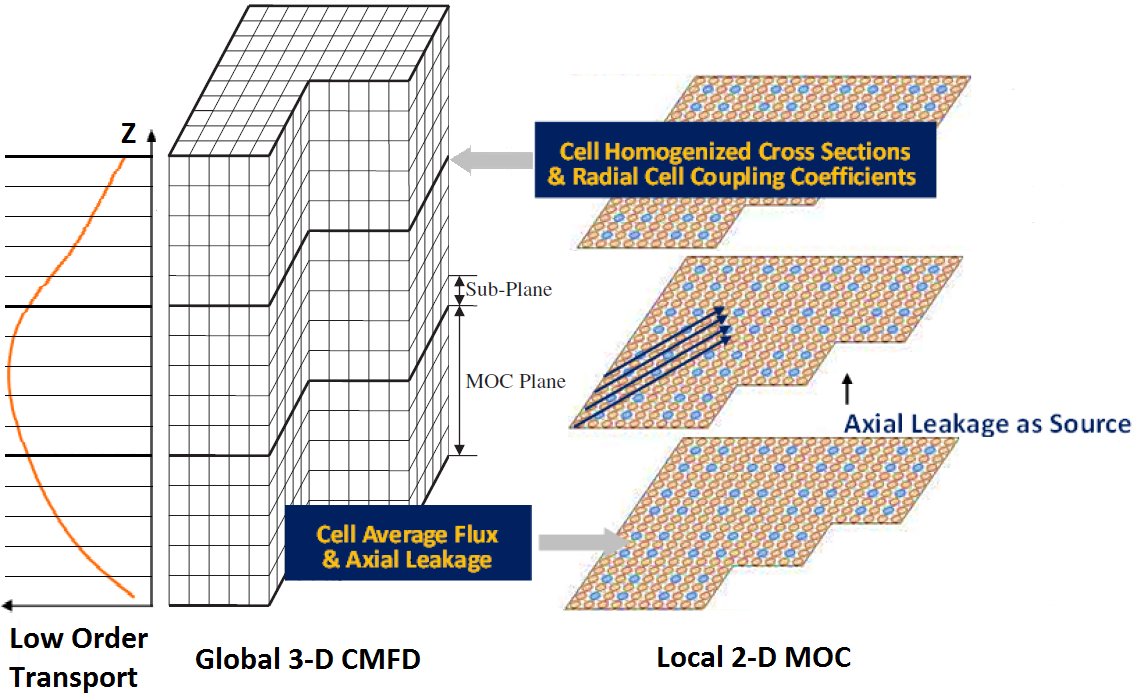
\includegraphics[width=0.8\textwidth]{../figs/2d1d-subplane.png}
    \caption[2D/1D Illustration]{The 2D/1D Method illustrated with the sub-plane scheme for the axial and CMFD calculations}
    \label{f:2d1dsubpalne}
\end{figure}

The second group of researchers was at Korea Atomic Energy Research Institute (KAERI).  They developed what is known more simply as the ``2D/1D'' scheme, first implemented in the DeCART code \cite{3DHetWholeCoreTransPlanarMOC,DeCARTTheoryManual,MethodsAndPerformanceOfDecart}.  This employs very similar technique to the 2D/1D Fusion method described above.  However, rather than using angular fluxes from each solver as a source term, currents are tallied on each of the six faces of each pin cell.  The currents can then be used to compute axial and radial ``transverse leakage'' sources for the radial and axial solvers, respectively.  This change allows for the storage of group-wise currents at each interface instead of storing the group-wise angular fluxes for each angle, significantly reducing the memory burden of the calculation.

After some development, the DeCART code was forked into several different versions for different institutions, one of them being the University of Michigan (UM).  After some development, it was determined that there would be no further development of the DeCART code at UM and a new 2D/1D implementation would be put in MPACT \cite{2D1DApproxTo3DTransport1,StabilityAndAccuracyOf3DTransportInMPACT}.  In MPACT's implementation of 2D/1D, 2D MOC is used for each of the radial planes, as with earlier 2D/1D codes.  The axial calculation done on a pin-homogenized mesh usually with SP$_3$, though a variety of other solver are available such as NEM, SENM, SP$_1$, SP$_5$, or S$_N$.  Finally, MPACT also uses 3D CMFD on the same pin-homogenized mesh to provide convergence acceleration to the calculations.  The remainder of this chapter will look at the derivation of the 2D/1D equations, the details of how they are implemented in MPACT, and some of the approximations and sources of errors related to this method.

\section{Derivation}

\subsection{Radial Equations}\label{ss:2d1dradialEq}

To derive the radial equations, we begin with the multigroup approximation in equation \ref{e:multigroupboltzmann}  and integrate in the $z$-direction over some range $\Delta z_i = z_{k+\frac{1}{2}} - z_{k-\frac{1}{2}}$.  To do this, we assume the cross-sections are all constant in the interval $z \in \left[z_{k-\frac{1}{2}},z_{k+\frac{1}{2}}\right]$.  With this assumption, we obtain the following equation:
\begin{subequations}
\begin{dmath}\label{e:2D1DradialEq}
{\Omega_x\frac{\partial \psi_{g}^Z}{\partial x} + \Omega_y\frac{\partial \psi_{g}^Z}{\partial y} + \frac{\Omega_z}{\Delta z_k}\left(\psi_{g,z_{k+\frac{1}{2}}} - \psi_{g,z_{k-\frac{1}{2}}}\right)} + {\Sigma_{t,g}\left(x,y\right)\psi_{g}^Z\left(x,y,\bm\Omega\right)} = {\frac{1}{4\pi}\sum_{g'=1}^{G}\intop_{4\pi}\Sigma_{s,g'\rightarrow g}^Z\left(x,y,\bm\Omega'\cdot\bm\Omega\right)\psi_{g'}^Z\left(x,y,\bm\Omega'\right)d\Omega'} + {\frac{1}{k_{eff}}\frac{\chi_{g}^Z}{4\pi}\sum_{g'=1}^G\intop_{4\pi} \nu\Sigma_{f,g'}^Z\left(x,y\right)\psi_{g'}^Z\left(x,y,\bm\Omega'\right)d\Omega'} + {\frac{Q_{g}^Z\left(x,y\right)}{4\pi}}
\end{dmath}
\begin{equation}
\psi_g^Z\left(x,y,\bm{\Omega}\right) = \frac{1}{\Delta z_k} \intop_{z_{k-\frac{1}{2}}}^{z_{k+\frac{1}{2}}} \psi_g^Z\left(x,y,z,\bm{\Omega}\right) dz
\end{equation}
\end{subequations}
where a superscript $Z$ indicates the average of a quantity over a given plane.  The $z$-component of the streaming can now be moved to the right-hand side of the equation and treated as a source term, giving a 2D transport problem which could be solved with a variety of methods:
\begin{subequations}
\begin{dmath}
{\Omega_x\frac{\partial \psi_{g}^Z}{\partial x} + \Omega_y\frac{\partial \psi_{g}^Z}{\partial y}} + {\Sigma_{t,g}\left(x,y\right)\psi_{g}^Z\left(x,y,\bm\Omega\right)} = {q_{g}^Z\left(x,y\right) + L_{g}^Z\left(x,y,\Omega_z\right)}
\end{dmath}
\begin{dmath}
q_{g}^Z\left(x,y\right) = {\frac{1}{4\pi}\sum_{g'=1}^{G}\intop_{4\pi}\Sigma_{s,g'\rightarrow g}^Z\left(x,y,\bm\Omega'\cdot\bm\Omega\right)\psi_{g'}^Z\left(x,y,\bm\Omega'\right)d\Omega'} + {\frac{1}{k_{eff}}\frac{\chi_{g}^Z}{4\pi}\sum_{g'=1}^G\intop_{4\pi} \nu\Sigma_{f,g'}^Z\left(x,y\right)\psi_{g'}^Z\left(x,y,\bm\Omega'\right)d\Omega'} + {\frac{Q_{g}^Z\left(x,y\right)}{4\pi}}
\end{dmath}
\begin{equation}
L_{g}^Z\left(x,y,\Omega_z\right) = \frac{\Omega_z}{\Delta z_k}\left(\psi_{g,z_{k-\frac{1}{2}}} - \psi_{g,z_{k+\frac{1}{2}}}\right)
\end{equation}
\end{subequations}
where $L_{g}^Z\left(x,y,\Omega_z\right)$ is the axial transverse leakage source term for plane $z$.  To simplify the source term, the axial transverse leakage term is often handled isotropically.  This is done by averaging over angle:
\begin{equation}
L_{g}^Z\left(x,y\right) = \frac{1}{4\pi}\intop L_{g}^Z\left(x,y,\Omega_z\right) \approx \frac{J_{g,z_{k-\frac{1}{2}}} - J_{g,z_{k+\frac{1}{2}}}}{4\pi\Delta z_k}
\end{equation}
where $J_{z_{i\pm \frac{1}{2}}}$ is the current at the top ($+$) or bottom ($-$) of the plane.  This eliminates the need for storing all the angluar fluxes on the top and bottom of every plane.  Other methods exist that allow the axial transverse leakage source to maintain its angular dependence without storing the angular fluxes \cite{KelleyBlakeThesis}, but these methods are not discussed here since they were not used by this work.

\subsection{Axial Equations}\label{ss:2d1daxialEq}

The axial equations can be derived in a manner similar to the radial equations.  Again, we begin with the multi-group approximation shown in equation \ref{e:multigroupboltzmann}.  This time, we integrate in both the x and y directions over intervals $x \in \left[x_{i-\frac{1}{2}},x_{i+\frac{1}{2}}\right]$ and $y \in \left[y_{j-\frac{1}{2}},y_{j+\frac{1}{2}}\right]$, giving the following equations in the axial direction, which are analogous to the radial equations in the previous section:
\begin{subequations}\label{e:2D1DaxialEq}
\begin{dmath}
{\Omega_z \frac{\partial \psi_{g}^{XY}}{\partial z}} + {\Sigma_{t,g}^{XY}\left(z\right)\psi_{g}^{XY}\left(z,\bm\Omega\right)} = q_{g}^{XY}\left(z,\Omega_x,\Omega_y\right) + {L_{g}^{XY}\left(z,\Omega_x,\Omega_y\right)}
\end{dmath}
\begin{dmath}
q_{g}^{XY}\left(z,\Omega_x,\Omega_y\right) = {\frac{1}{4\pi}\sum_{g'=1}^G\intop_{4\pi} \Sigma_{s,g'\rightarrow g}^{XY}\left(z,\bm\Omega'\cdot\bm\Omega\right)\psi_{g'}^{XY}\left(z,\bm\Omega'\right)d\Omega'} + {\frac{1}{k_{eff}}\frac{\chi_{g}^{XY}}{4\pi}\sum_{g'=1}^G\intop_{4\pi}\nu\Sigma_{f,g'}^{XY}\left(z\right)\psi_{g'}^{XY}\left(z,\bm\Omega'\right)d\Omega'} + {\frac{Q_{g}^{XY}\left(z\right)}{4\pi}}
\end{dmath}
\begin{dmath}
L_{g}^{XY}\left(z,\Omega_x,\Omega_y\right) = {\frac{\Omega_x}{\Delta y_i}\intop_{y_{i-\frac{1}{2}}}^{y_{i+\frac{1}{2}}} \left(\psi_{g,x_{i-\frac{1}{2}}}\left(y\right) - \psi_{g,x_{i+\frac{1}{2}}}\left(y\right) dy\right)} + {\frac{\Omega_y}{\Delta x_i}\intop_{x_{i-\frac{1}{2}}}^{x_{i+\frac{1}{2}}} \left(\psi_{g,y_{i-\frac{1}{2}}}\left(x\right) - \psi_{g,y_{i+\frac{1}{2}}}\left(x\right) dx\right)}
\end{dmath}
\begin{equation}\label{e:2D1DaxFluxDef}
\psi_g^{XY} = \frac{1}{\Delta_i \Delta_j} \intop_{y_{j-\frac{1}{2}}}^{y_{j+\frac{1}{2}}} \intop_{x_{i-\frac{1}{2}}}^{x_{i+\frac{1}{2}}} \psi_g\left(x,y,z,\bm{\Omega}\right) dx dy
\end{equation}
\end{subequations}
where a superscript $XY$ now corresponds to a particular x- and y-region which extends the full height of the problem in the z-direction.  Again, it is assumed that the cross-sections are constant in the x- and y-directions inside the region of integration.  How this is accomplished will be discussed in more detail when discussing MPACT's implementation of SP$_3$ and CMFD.

As with the radial equations, we can treat the transverse leakage source isotropically by averaging over angle:

\begin{dmath}
{L_{g}^{XY}\left(z\right)} = {\frac{1}{4\pi}\intop_{4\pi} L_{g}^{XY}\left(z,\Omega_x,\Omega_y\right)} \approx {\frac{1}{4\pi\\Delta y_i}\intop_{y_{i-\frac{1}{2}}}^{y_{i+\frac{1}{2}}}\left( J_{g,x_{i-\frac{1}{2}},y_i}\left(z\right) - J_{g,x_{i+\frac{1}{2}},y_i}\left(z\right)\right)dy} + {\frac{1}{4\pi\Delta x_i}\intop_{x_{i-\frac{1}{2}}}^{x_{i+\frac{1}{2}}}\left( J_{g,x_i,y_{i-\frac{1}{2}}}\left(z\right) - J_{g,x_i,y_{i+\frac{1}{2}}}\left(z\right)\right)dx}
\end{dmath}

Again, methods have been developed to angle the angle-dependence of the radial transverse leakage source \cite{StimpsonShaneThesis}, but this work used only isotropic radial leakage.

\section{Implementation}

\begin{figure}[h]
  \centering
  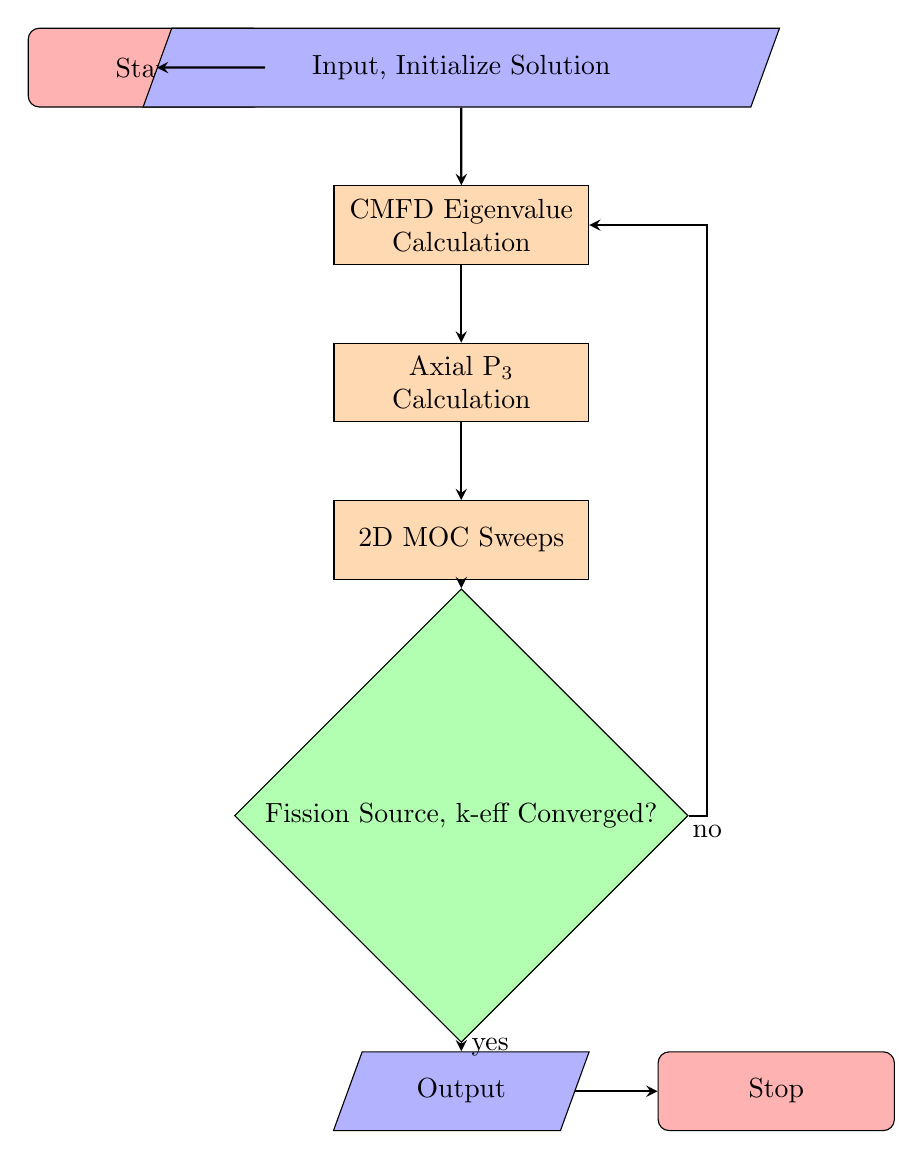
\begin{tikzpicture}[node distance=2cm]

% Begin
\node (start) [startstop] {Start};
\node (init) [io, right of=start, xshift=2.0cm] {Input, Initialize Solution};

% CMFD
\node (CMFD) [process, below of=init] {CMFD Eigenvalue Calculation};

% Nodal
\node (Nodal) [process, below of=CMFD] {Axial P$_3$ Calculation};

% MOC
\node (MOC) [process, below of=Nodal] {2D MOC Sweeps};

% Finish
\node (convCheck) [decision, below of=MOC, yshift=-1.5cm] {Fission Source, k-eff Converged?};
\node (out) [io, below of=convCheck,yshift=-1.5cm] {Output};
\node (stop) [startstop, right of=out, xshift=2.0cm] {Stop};

% Basic Arrows
\draw [arrow] (start) -- (init);
\draw [arrow] (init) -- (CMFD);
\draw [arrow] (CMFD) -- (Nodal);
\draw [arrow] (Nodal) -- (MOC);
\draw [arrow] (MOC) -- (convCheck);
\draw [arrow] (out) -- (stop);

% Fancy Arrows
\draw [arrow] (convCheck) -- node[anchor=west] {yes} (out);
\draw [arrow] (convCheck) -| node[anchor=north] {no} ([xshift=1.5cm]Nodal.east) |- (CMFD);

\end{tikzpicture}
  \caption{Calculation flow for 2D/1D scheme}\label{f:2d1d-flowchart}
\end{figure}

Now that the general 2D/1D scheme has been described, some attention should be given to the details of its implementation in MPACT.  Figure \ref{f:2d1d-flowchart} shows the calculation flow used by MPACT.  The first step is to perform a global 3D CMFD calculation to obtain pin-averaged flux and interface currents between each cell.  Next, the axial solver uses the radial currents calculated by CMFD as a radial transverse leakage source to obtain an axial transverse leakage source for the radial solver.  Finally, 2D MOC is used as the radial solver to obtain a solution with sub-pin resolution in each plane.

\subsection{3D Sub-plane CMFD}\label{ss:2d1d-3dcmfd}

The CMFD method was originally implemented in MPACT just as described in section \ref{ss:CMFD}.  To do this, each pin cell is homogenized using the quantities defined in equation \ref{e:CMFDhomogTerms} in every plane in the model.  The radial coupling coefficients defined in equation \ref{e:CMFDcouplingCoeffs} are obtained by calculating the current at the interface between each pair of pin cells using the 2D MOC sweeper, while the axial coupling coefficients are obtained from the axial currents calculated by the axial solve during the previous iteration.  The matrix for the 3D multi-group system can then be set up and solved, typically using the generalized Davidson eigenvalue solver.

In addition to this traditional 3D CMFD, MPACT also has the capability to use the sub-plane scheme.  This scheme was first developed by Cho et al. for the DeCART code \cite{DeCARTsubplane}.  Thin MOC planes are capable of causing instability in the 2D/1D scheme, but are sometimes required to maintain accuracy.  The sub-plane scheme allows users to increase the thickness of the 2D planes while still maintaining the accuracy of a fine axial mesh.  Later, the developers of the nTRACER code \cite{RyuBEAVRSnTRACER2015} also used the sub-plane scheme.  In addition to how it was used in DeCART, nTRACER also uses the sub-plane scheme as part of its rod decusping methods \cite{ICAPPcontrolRodDecuspingNTRACER}.  MPACT also uses sub-plane as part of a decusping treatment, which will be discussed in greater detail in chapter \ref{chap:cusping}.  This section will deal only with the basics of the sub-plane method as it was used in DeCART.


\subsubsection{Homogenization}

The difference between the sub-plane scheme and traditional CMFD is that the CMFD system is that the CMFD system is allowed to have multiple axial planes for each of the 2D planes in which the transport calculations are done.  This allows CMFD to capture sub-plane axial flux shapes that would otherwise be ignored.  To do this, a sub-plane scaling factor is introduced which will be used to provide an axial shape within a 2D plane:

\begin{align}
c_{g,i}^k &= \frac{\phi_{g,i}^{k-1}}{\overline{\phi}_{g,i}^{k-1}} \nonumber\\
 &= \frac{\phi_{g,i}^{k-1} \sum_{i'=1}^{N_{sp}} V_{i'}}{\sum_{i'=1}^{N_{sp}} \phi_{g,i'}^{k-1} V_{i'}}
\end{align}

where superscripts indicate which iteration the values are taken from and $N_{sp}$ is the number of sub-planes for the pin cell of interest.  Now when the homogenized values are calculated from the 2D transport solution using equation \ref{e:CMFDhomogTerms}, the fine mesh flux is multiplied by this sub-plane scaling factor everywhere it appears.  Because the 2D/1D scheme assumes a constant material axially in each plane, this sub-plane factor has no impact on the homogenized cross-sections.  However, the homogenized flux $\phi_{g,i}$ and fission source distribution $\chi_{g,i}$ will be changed, providing an axial shape for the source term in the eigenvalue calculation.

\subsubsection{Coupling Coefficients}

In addition to the homogenized cell terms, the coupling coefficients described by equations \ref{e:CMFDinterface} and \ref{e:CMFDcouplingCoeffs} must be calculated for each sub-plane.  To maintain consistency, the area-averaged current calculated by the radial sweeper must be preserved across the sub-surfaces used by the sub-plane scheme.  Thus, the current calculated by the radial sweeper at an interface is used at the corresponding interfaces for all sub-planes in that plane.  Additionally, to maintain consistency, this requires that the cell-homogenized flux used in the calculation of the diffusion coefficients be defined for the entire MOC plane as in equation \ref{e:CMFDhomogFlux} rather than using the sub-plane scaling factor for each sub-plane.

The axial coupling coefficient can be treated in a more straightforward manner.  Because the 1D axial solvers use the same pin-homogenized mesh as the CMFD solver, axial currents are naturally calculated at the top and bottom of each of the sub-planes.  Thus, these currents can be used together with the sub-planes fluxes to calculate sub-plane--dependent axial coupling coefficients.

\subsubsection{Projection}

The projection of the CMFD flux back to the 2D planes must also account for the presence of the sub-planes.  To do this, the solution is volume-averaged over all sub-planes for each pin cell, resulting in an equation similar to \ref{e:CMFDscaling}:

\begin{equation}
\phi_{trans,g,j}^k = \frac{\sum_{i'=1}^{N_{sp}} \phi_{CMFD,g,i'}^k V_i}{\sum_{i'=1}^{N_{sp}} \phi_{CMFD,g,i'}^k V_i} \phi_{trans,g,j}^{k-1}
\end{equation}

The calculation flow for 3D CMFD is shown in figure \ref{f:CMFD-flowchart}.

\begin{figure}[h]
  \centering
  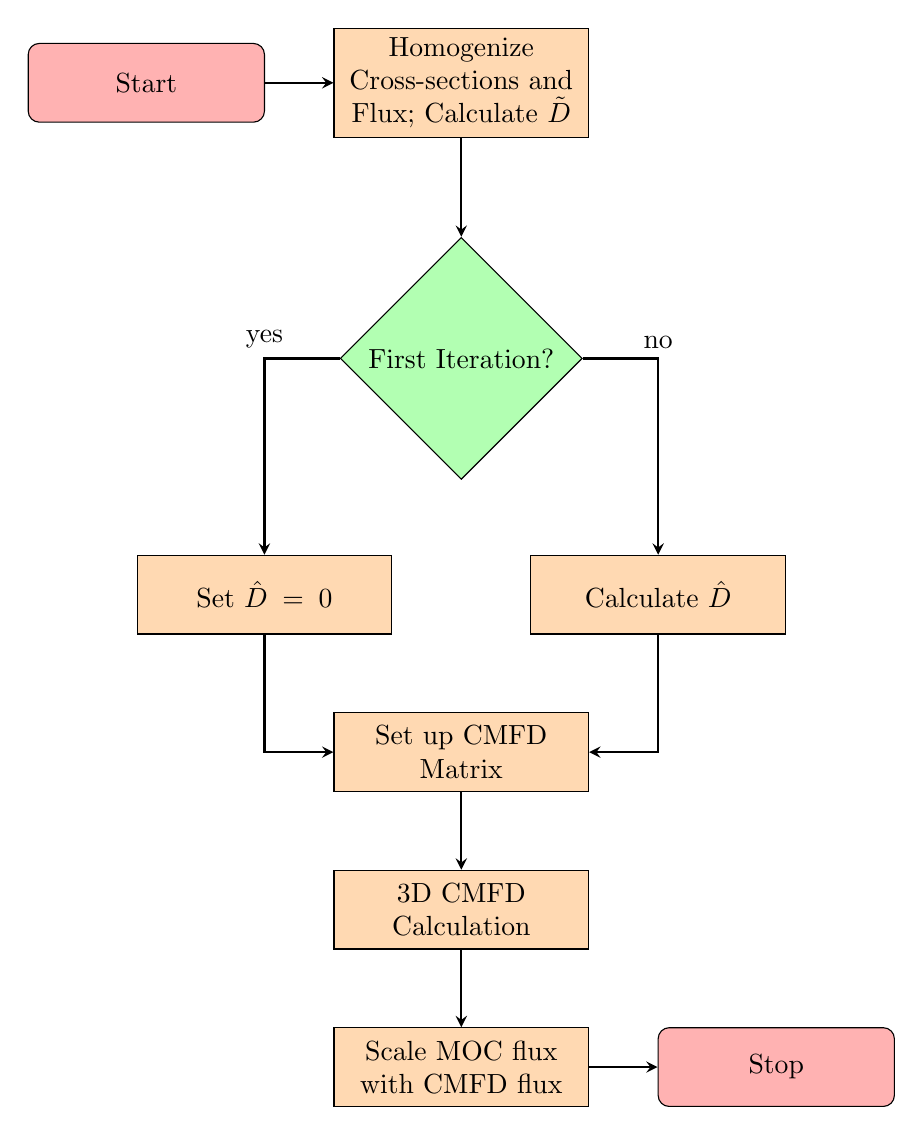
\begin{tikzpicture}[node distance=2cm]

% Start
\node (start) [startstop] {Start};

% CMFD
\node (homog) [process, right of=start, xshift=2.0cm] {Homogenize Cross-sections and Flux; Calculate $\tilde{D}$};
\node (iterCheck) [decision, below of=homog, yshift=-1.5cm] {First Iteration?};
\node (firstIter) [process, below of=iterCheck, xshift=-2.5cm, yshift=-1.0cm] {Set $\hat{D}=0$};
\node (laterIter) [process, below of=iterCheck, xshift=2.5cm, yshift=-1.0cm] {Calculate $\hat{D}$};
\node (matrix) [process, below of=firstIter, xshift=2.5cm] {Set up CMFD Matrix};
\node (3DCMFD) [process, below of=matrix] {3D CMFD Calculation};
\node (proj) [process, below of=3DCMFD] {Scale MOC flux with CMFD flux};

% Stop
\node (stop) [startstop, right of=proj, xshift=2.0cm] {Stop};

% Basic Arrows
\draw [arrow] (start) -- (homog);
\draw [arrow] (homog) -- (iterCheck);
\draw [arrow] (matrix) -- (3DCMFD);
\draw [arrow] (3DCMFD) -- (proj);
\draw [arrow] (proj) -- (stop);

% Fancy Arrows
\draw [arrow] (iterCheck) -| node[anchor=south] {yes} (firstIter);
\draw [arrow] (iterCheck) -| node[anchor=south] {no} (laterIter);
\draw [arrow] (firstIter) |- (matrix);
\draw [arrow] (laterIter) |- (matrix);

\end{tikzpicture}
  \caption{Calculation flow for 3D sub-plane CMFD}\label{f:CMFD-flowchart}
\end{figure}

\subsection{1D SP\textsubscript{3}}

In MPACT, the 1D axial solvers operate on the same mesh as the 3D CMFD calculations, meaning that cell-homogenized quantities and radial currents have already been obtained from the CMFD calculation.  All the 1D axial solver must do is construct a source term from the radial currents for each cell, then perform a calculation to obtain currents on the axial interfaces at the top and bottom of each node.

MPACT has a variety of 1D nodal methods that are capable of performing these calculations, including diffusion-based such as NEM and SENM and higher-order solvers such as SP$_N$ and S$_N$.  For most MPACT calculations, including those in this work, the solver of choice is SP$_3$, which provides significant improvement over the diffusion-based methods and SP$_1$.  Very little benefit is obtained by using the higher-order SP$_5$.

\begin{figure}[h]
  \centering
  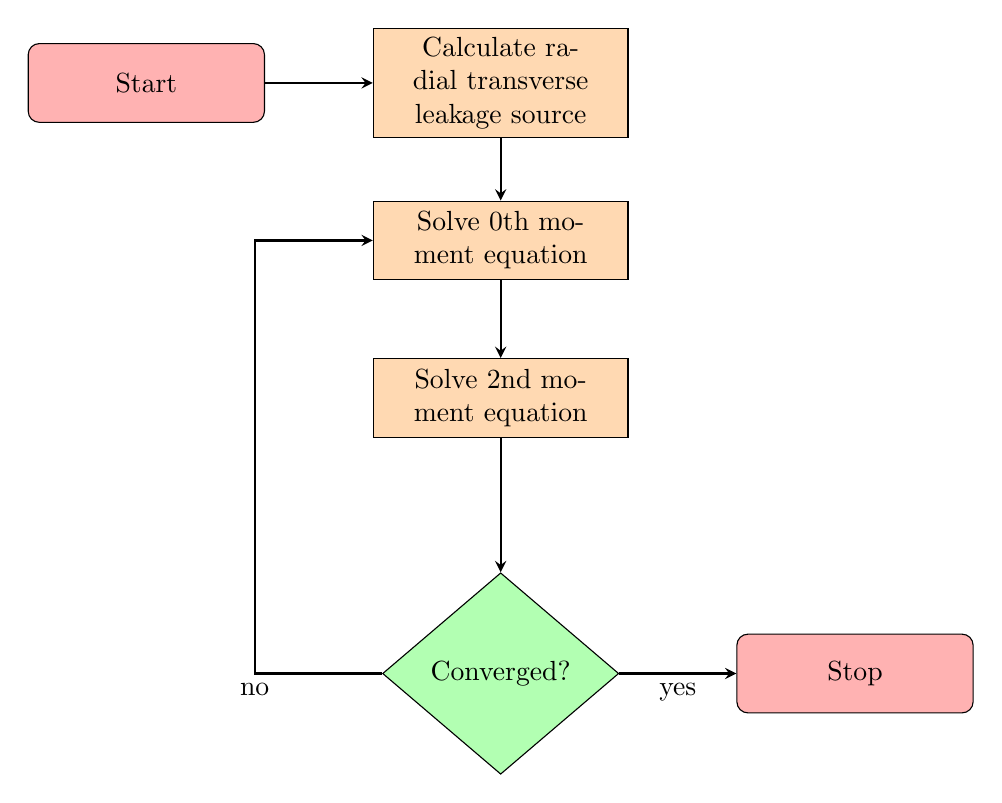
\begin{tikzpicture}[node distance=2cm]

% Begin
\node (start) [startstop] {Start};

% Nodal
\node (radialTL) [process, right of=start, xshift=2.5cm] {Calculate radial transverse leakage source};
\node (sp3-0) [process, below of=radialTL] {Solve 0th moment equation};
\node (sp3-2) [process, below of=sp3-0] {Solve 2nd moment equation};
\node (convCheck) [decision, below of=sp3-2, yshift=-1.5cm] {Converged?};

% Stop
\node (stop) [startstop, right of=convCheck, xshift=2.5cm] {Stop};

% Basic Arrows
\draw [arrow] (start) -- (radialTL);
\draw [arrow] (radialTL) -- (sp3-0);
\draw [arrow] (sp3-0) -- (sp3-2);
\draw [arrow] (sp3-2) -- (convCheck);
\draw [arrow] (convCheck) -- node[anchor=north] {yes} (stop);

% Fancy Arrows
\draw [arrow] (convCheck) -| node[anchor=north] {no} ([xshift=-1.5cm]sp3-2.west) |- (sp3-0);

\end{tikzpicture}
  \caption{Calculation flow for 1D axial calculations in MPACT}\label{f:Axial-flowchart}
\end{figure}

The SP$_3$ equations consist of equations for angular flux moments 0 through 3.  These equations can be combined into two equations for just the 0th and 2nd moments.  With the equations formulated this way, MPACT can iterate between the two moments until they converge, then calculate axial currents and move on to the radial calculations.

While SP$_3$ handles the angle dependence of the flux, it does not handle the spatial dependence.  To do this, the SP$_3$ solvers are wrapped in a two-node NEM solver.  This method assumes that the flux has a fourth-order polynomial shape in space and that the source term has a second-order shape.  Using the neighboring cells above and below each cell, this source term shape is constructed and used to solve for the 0th moment of the flux.

\subsection{2D MOC}

For the radial calculations, 2D MOC is used.  This allows MPACT to easily calculate scalar fluxes and currents in each plane regardless of the geometric complexity.  This section is devoted to discussing some of the details of the MOC implementation and sweeping algorithm in MPACT.

\subsubsection{Ray Tracing}

\begin{figure}[h]
    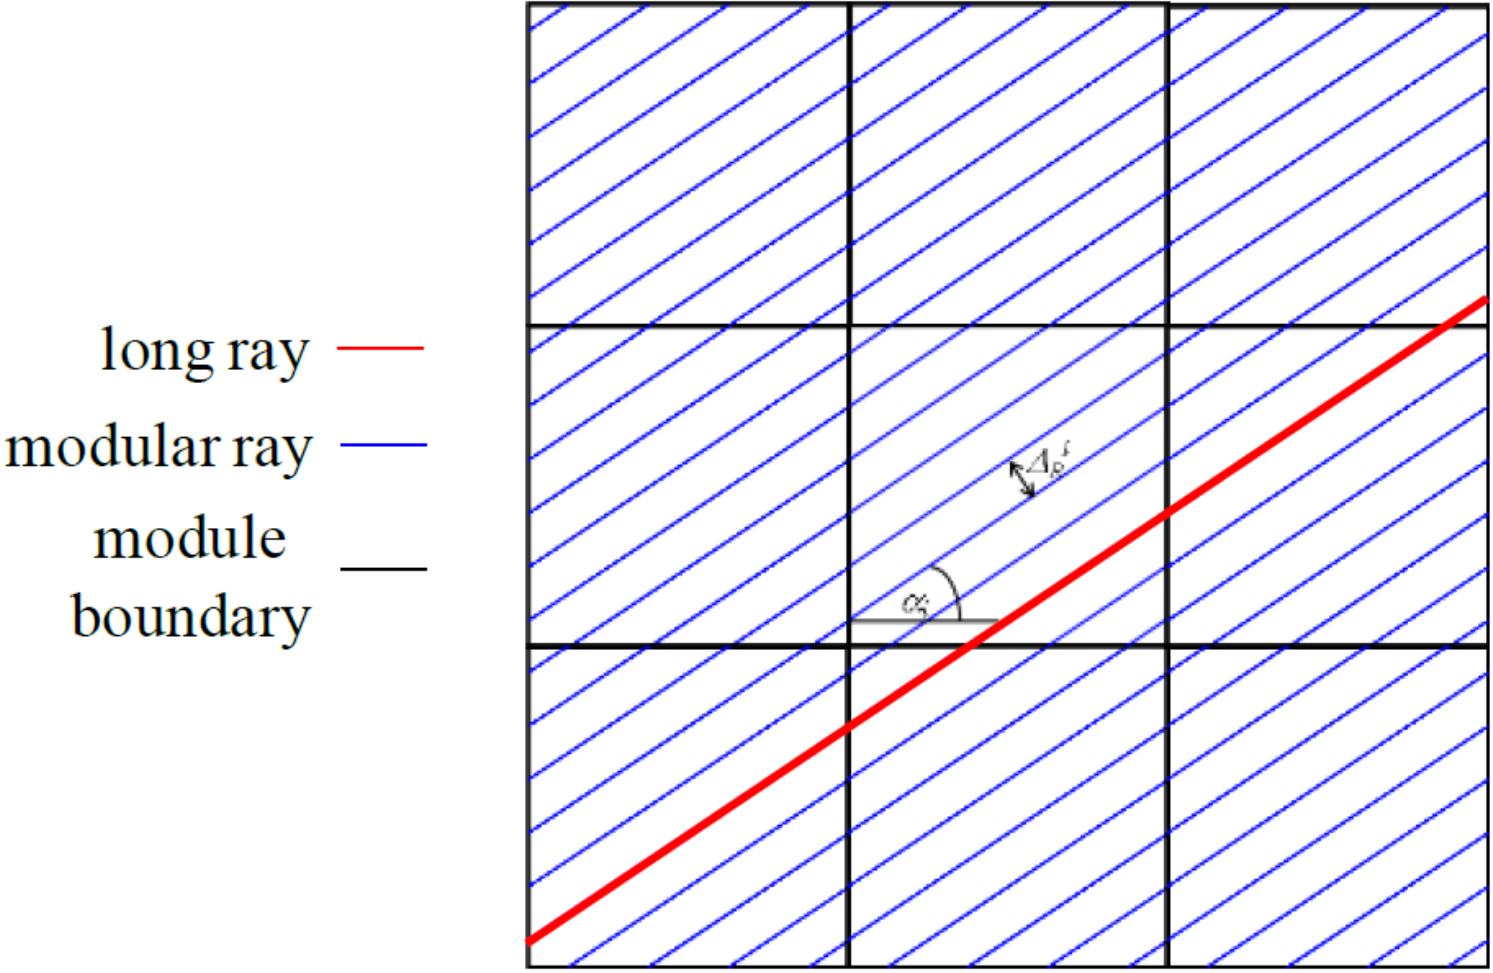
\includegraphics[width=0.5\textwidth]{modular_rays.png}
    \caption[Modular Ray Tracing]{Modular ray tracing depiction \cite{MPACTTheoryManual}}\label{e:ModRays}
\end{figure}

One of the key features of MPACT's MOC implementation is that of modular ray tracing.  Ray tracing is performed once at the beginning of a calculation and stored for the remainder of the calculation.  Doing this greatly reduces the runtime of the MOC sweeps since the length of each ray segment and the region it is crossing are already known ahead of time.  Furthermore, MPACT takes advantage of the repeatable nature of a reactor's geometry.  Because reactor geometry is repetitive, small portions of the geometry which repeat frequently can be ray-traced separately instead of tracing the entire core.  These smaller units of geometry are known as ray tracing modules, and in MPACT can be a full fuel assembly, a quarter fuel assembly, or a single fuel pin.  After the unique modules are identified, each of them is ray-traced in such a way that the endpoints of a ray in each module will line up with the beginning of a ray in the neighboring module.  This significantly reduces the storage requirements for the ray data since a small number of ray tracing modules can represent a full core problem.

As a result of the modular ray tracing, several corrections are required.  First, to successfully perform the ray tracing the angles of the rays had to be adjusted slightly to line up.  However, because a quadrature is used to integrate the angular flux, this angle modification requires a correction to the quadrature weights as well to maintain accuracy.  Second, the spacing between the rays must also be adjusted slightly to ensure that all rays align.  Along with these corrections, there are other MOC concepts such as volume corrections, cyclic rays, and others which are important to be aware of but will be deferred to the MPACT theory manual for details \cite{MPACTTheoryManual}.

\subsubsection{Sweeping Algorithm}\label{sss:2d1dMOCsweepAlgorithm}

\begin{figure}[h]
  \centering
  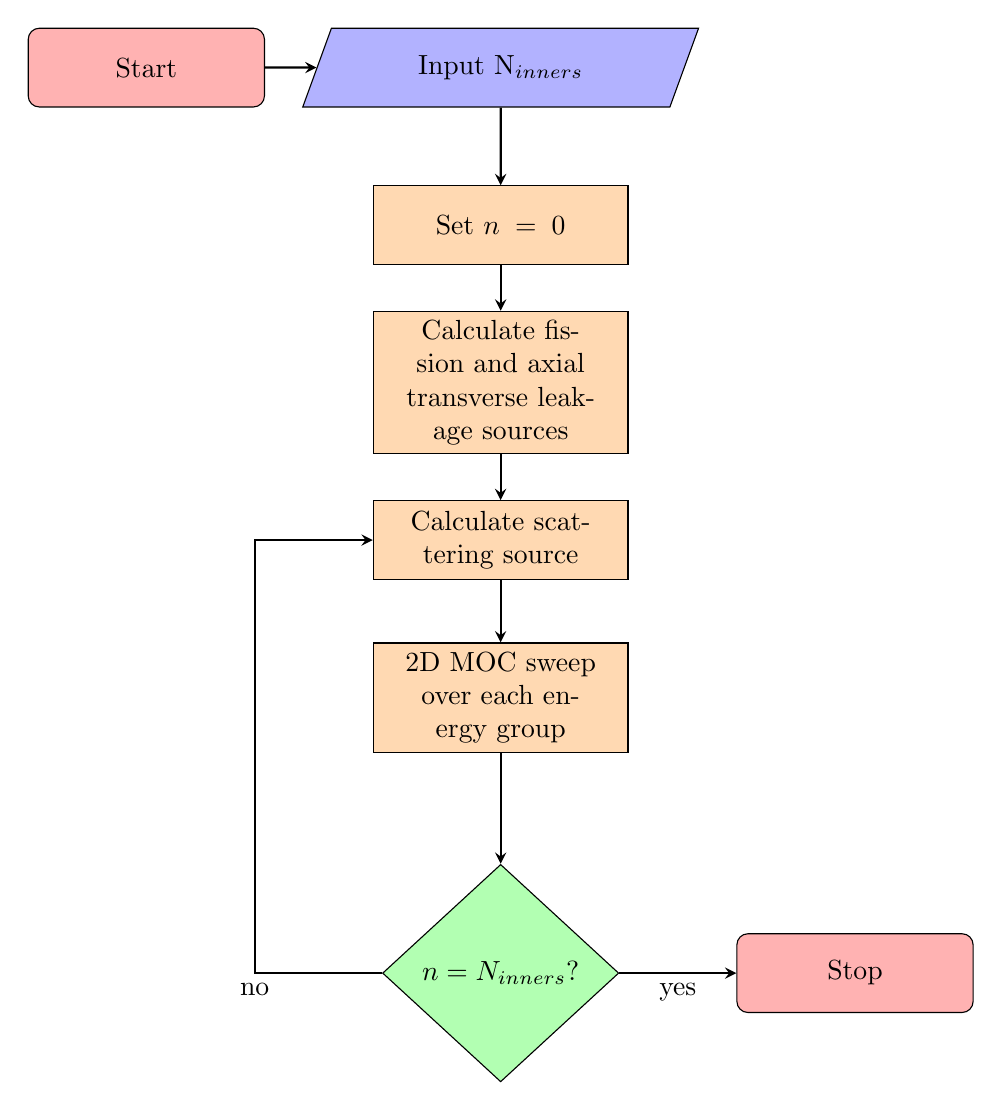
\begin{tikzpicture}[node distance=2cm]

% Begin
\node (start) [startstop] {Start};
\node (init) [io, right of=start, xshift=2.5cm] {Input N$_{inners}$};

% MOC
\node (begin) [process, below of=init] {Set $n=0$};
\node (source) [process, below of=begin] {Calculate fission and axial transverse leakage sources};
\node (scatSource) [process, below of=source] {Calculate scattering source};
\node (MOC) [process, below of=scatSource] {2D MOC sweep over each energy group};
\node (MOCdone) [decision, below of=MOC, yshift=-1.5cm] {$n = N_{inners}$?};z
\node (stop) [startstop, right of=MOCdone, xshift=2.5cm] {Stop};

% Basic Arrows
\draw [arrow] (start) -- (init);
\draw [arrow] (init) -- (begin);
\draw [arrow] (begin) -- (source);
\draw [arrow] (source) -- (scatSource);
\draw [arrow] (scatSource) -- (MOC);
\draw [arrow] (MOC) -- (MOCdone);

% Fancy Arrows
\draw [arrow] (MOCdone) -| node[anchor=north] {no} ([xshift=-1.5cm]MOC.west) |- (scatSource);
\draw [arrow] (MOCdone) -- node[anchor=north] {yes} (stop);

\end{tikzpicture}
  \caption{Calculation flow for 2D MOC calculation in MPACT}\label{f:MOC-flowchart}
\end{figure}

To perform the MOC sweeps, MPACT uses a multi-group sweeping method.  To do this, multi-group sources and cross-sections are prepared for each of the fine mesh regions in each plane.  There are then four total loops for the sweeping algorithm.  From outermost to innermost, these loops are over azimuthal angle, ray (across the entire domain), polar angle, and energy group.  Each ray is divided into many segments that the MOC steps its way along as described in section \ref{ss:MOCtheory}.  As these sweeps are performed, scalar flux is tallied in each fine mesh region, and, assuming CMFD is being used, currents are tallied at the interfaces between each pin cell.  Normally only one inner MOC iteration is required per 2D/1D iteration.  This algorithm is shown in figure \ref{f:MOC-flowchart}.

MPACT also has the capability of performing the MOC sweeps with the energy loop as the outermost.  This has two advantages.  First, the previous group is used to construct the scattering source for the current group.  This means that the iteration scheme is a Gauss-Seidel iteration instead of a Jacobi iteration, which can speed up the convergence of the problem.  Secondly, the cross-sections and sources only need to be stored for one group at a time, minimizing the storage requirements for the calculations.  However, when using transport-corrected cross-sections, some instabilities have been observed in this iteration scheme when using only a single inner iteration.  Further more, having the energy loop on the inside results in some improved cache efficiency when it comes to traversing the rays, reducing the runtime for a single MOC sweep \cite{JacobiInscatterTechReport}.  For these two reasons, MPACT defaults to the Jacobi-style iteration scheme described first.

\section{Parallel Decomposition}

While the 2D/1D scheme greatly reduces runtime from a direct 3D transport calculation, it is still computationally expensive when compared to nodal methods traditionally used by industry.  To minimize the walltime required for 2D/1D calculations in MPACT, several different methods of decomposing the problem for parallel execution have been implemented.  These methods allow MPACT to easily scale to hundreds or thousands of CPUs.  Each of these methods will be briefly described in this section.

\begin{enumerate}[leftmargin=*]
\item \textbf{Spatial Decomposition}

When using this decomposition, each parallel process only has a portion of the model.  Each portion is solved locally by one process, then boundary data is communicated to all processes which own neighboring portions of the model.  The updated boundary data is then used in the following iteration.  When using spatial decomposition, planar decomposition is performed first.  This means that if the total number of parallel processes being used is less than or equal to the number of 2D MOC planes, then one or more entire planes is simulated by each process.  If more processes are used than there are planes in the model, then radial decomposition is performed.  This decomposes every plane radially into smaller pieces.  Every plane must be radially decomposed in the same way, and the smallest unit allowed in radial decomposition is a single ray-tracing module.  Because spatial decomposition does not duplicate much memory and does not decrease the computational efficiency significantly, it is usually the preferred choice of decomposition methods.

\item \textbf{Angle Decomposition}

For angle decomposition, each process has the entire spatial domain.  When the MOC sweeps are performed, each process only sweeps a subset of the angles in the selected quadrature.  After the sweep, a reduction is performed to get the actual scalar flux and currents on all processes.  For the CMFD calculation, the angle processes are re-purposed as spatial processes.  Each angle process owns the full domain, but only solves a portion of it as if it were spatially decomposed.

It is possible to use both spatial and angle decomposition together.  When this is done, spatial decomposition is performed first, then angle decomposition is done within each spatial domain.  In general, the efficiency of angle decomposition calculations is less than that of spatial decompositions.  Furthermore, it also requires that each angle process models all of the spatial domain, increasing the total memory required for the calculation compared with finer spatial decomposition.  However, angle decomposition is still useful for reducing the runtime of cases where further spatial decomposition is not possible.

\item \textbf{Ray Decomposition}

A third type of decomposition that can be done is to decompose the rays in the MOC calculation.  Unlike the previous methods, the ray decomposition makes use of shared-memory threading instead of distributed memory message passing.  While performing the MOC sweeps, several threads are used to solve all the rays in each angle.  For the CMFD calculation, MPACT has internal RBSOR solvers which are capable of using threading.  However, when third-party libraries are used for the CMFD calculations, the threading will be used only during the CMFD calculation.  Threading can also be combined with both spatial and angle decomposition to further increase the parallelism of MPACT.

\item \textbf{Energy Decomposition}

At this time, energy decomposition is not available in MPACT.  However, when it is added, it will be similar to the angle decomposition.  For the MOC calculation, each process will solve a subset of the energy groups on the spatial domain, and for the CMFD calculation, the energy processes will be re-purposed as space processes.
\end{enumerate}

\section{Sources of Error}\label{s:2d1dErrors}

The 2D/1D approximation as several sources of error.  Some of these are addressed by mesh, ray spacing, or quadrature refinements, but others are due to approximations made in the method itself.  The sources of error which are due to fundamental approximations in the 2D/1D method will be discussed first, followed by a brief (not comprehensive) list of some other common sources of error.

\subsection{Axial Homogenization}

When deriving the radial equations in section \ref{ss:2d1dradialEq}, it was assumed that the cross-sections were constant in the axial direction for each of the planes.  While this is often the case if an appropriate axial mesh is selected, sometimes it is impractical to mesh the problem finely enough to ensure this.  When an axial material heterogeneity is present in a plane, 2D MOC requires that these materials be homogenized.  In some cases, a simple volume-averaging is sufficient, but if a material with a large cross-section is being homogenized with a material that has a significantly different cross-section, significant errors can result.  To prevent this without refining the axial mesh, some modification to the 2D/1D scheme is required to improve the homogenization.  This will be addressed in chapter \ref{chap:cusping}.

\subsection{Axial Transverse Leakage Source}

Another approximation relates to the assumptions made while deriving the axial equations in section \ref{ss:2d1daxialEq}.  The SP$_3$ calculations are performed on a pin-homogenized mesh.  Because of this, the axial currents used in the axial TL source are assumed to be flat across the entire pin cell.  However, the currents will obviously be quite different in the fuel and moderator regions.  Furthermore, the axial TL is treated isotropically.  While this simplifies the axial calculations and MOC storage requirements, it does not perfectly reflect reality.  Both these spatial and angular assumptions introduce some error into the axial TL source used by MOC.

\subsection{Radial Currents}

The radial TL source used by the axial SP$_3$ solver has the same two approximations as the axial TL source did.  Radial currents are used to generate the source, which assumes isotropy.  Additionally, the spatial shape is flat across each pin cell.  This is corrected to some extent since the axial solver produces a quadratic source shape using the neighboring nodes, but this is not a perfect solution.

Additionally, when using the sub-plane method, the $\hat{D}$ correction terms used by CMFD are assumed to be axially flat within each MOC plane.  While this assumption improves the stability of the calculations, it forces CMFD to capture any axial shape the current has within an MOC plane.  For most problems, this error is probably negligible, but for cases such as a partially inserted rod or other strong absorber, it would be beneficial to be able to have sub-plane--dependent $\hat{D}$ terms to more accurately calculate the radial currents.  Doing this would improve the radial TL source in the SP$_3$ solver, and the the overall 2D/1D results.

\subsection{Other Sources of Error}

Several other sources of error in the 2D/1D method will be briefly mentioned here, but not discussed in detail.

\begin{enumerate}[leftmargin=*]
  \item \textbf{Ray Spacing}
  
  The spacing between the rays in the MOC calculation is important to the accuracy of the calculation.  At minimum, one ray needs to pass through each of the fine mesh regions, but multiple rays will improve the accuracy.  A typical ray spacing is 0.05 cm, but sometimes finer spacing may be required.
  
  \item \textbf{Radial Meshing}
  
  The radial and azimuthal meshing of each of the pin cells must be fine enough to give a good solution.  In MPACT, fuel pins usually have 3 radial rings, with an extra ring in the moderator region to resolve the change in the flux near the edge of the fuel pin.  Each ring is typically divided into 8 azimuthal regions.
  
  \item \textbf{Axial Meshing}
  
  The axial mesh must be refined enough to capture the axial shape of the solution.  Usually MOC planes of about 8 cm thick are used for a typical PWR calculation, which some thinner planes to resolve spacer grids, burnable poison inserts, or other components.  Using thicker planes could decrease accuracy and worsen the convergence of the calculation.
  
  \item \textbf{Scattering Treatment}
  
  Scattering in a reactor, especially off the hydrogen atoms in the moderator, is anisotropic.  To resolve this, a sufficiently high-order scattering treatment must be used in the MOC calculations.  For PWRs, $P_1$ to $P_3$ is a typical range.  MPACT is capable of going up to P$_5$ scattering treatment for libraries which have the required data.
  
  An alternative is to use transport-correction P$_0$ scattering.  This can capture the anisotropy without increasing the runtime of the calculations.  However, there are several methods of calculating the transport cross-sections, and none of them are perfect.  Thus, using the TCP$_0$ option in MPACT also has some non-trivial error associated with it.
  
  \item \textbf{Cross-Section Library}
  
  To perform any calculations using the 2D/1D method, a multi-group cross-section library must be available.  While this is not technically a source of error in the 2D/1D method itself, the cross-section library can be difficult to generate correctly.  Any error in any isotope in the library will cause error in the 2D/1D calculations if the isotope is used in the model.  Thus, the 2D/1D method is useless if the a bad cross-section library is being used.
  
  \item \textbf{Self-Shielding}
  
  Another potential source of error is related to spatial and energy self-shielding.  To correctly deal with resonance absorption in the fuel while also accounting for the spatial self-shielding in the fuel, MPACT uses the subgroup method \cite{SubgroupOrig1974,SelfShieldingMethodologyMPACT2013}.  Without using this method, the k$_{eff}$ calculated by MPACT is off by several percent, along with an inaccurate flux distribution.
  
  \item \textbf{Quadrature}
  
  One final source of error that can arise is in the selection of a quadrature.  It is important to select both an appropriate number of azimuthal and polar angles as well as an appropriate type of quadrature.  Typically around 16 azimuthal angles and 3 polar angles is sufficient.  There are several different types of quadratures implemented in MPACT, but generally a Tabuchi-Yamamoto quadrature is used for the polar angles \cite{YamamotoQuadrature2012} with a Chebyshev quadrature for the azimuthal angles \cite{HandbookOfMathFunctions1972}.
\end{enumerate}

\chapter{Rod Cusping}
This chapter will focus specifically on control rod cusping effects, which are the focus of this work.  First, a more thorough definition of the problem and motivation for solving it will be presented.  The next section will then present some of the solutions that have been used to minimize the cusping effects in the past, including a simplified decusping model implemented in MPACT itself.  The third section will then discuss some newer methods based on the sublpane CMFD scheme that have recently been implemented in MPACT.  Finally, a new ``sub-ray'' MOC method will be proposed to deal with the cause of the cusping effects on a more fundamental level.

\section{Background}

In Section \todo{section num}, some potential sources of errors for the 2D/1D scheme were introduced.  One of these was the error introduced by axial homogenization within a 2D MOC plane.  In some cases, this can be done without introducing significant errors.  For example, MPACT often homogenizes components outside the active fuel region, such as the end plugs and gaps at the end of the fuel rods.  However, when strong neutron absorbers, such as control rods, are homogenized axially in active fuel region, this has the effect of introducing absorption in regions where there should be none.  This effect is known as ``cusping,'' and is illustrated in Figure 

\begin{figure}
    \centering
    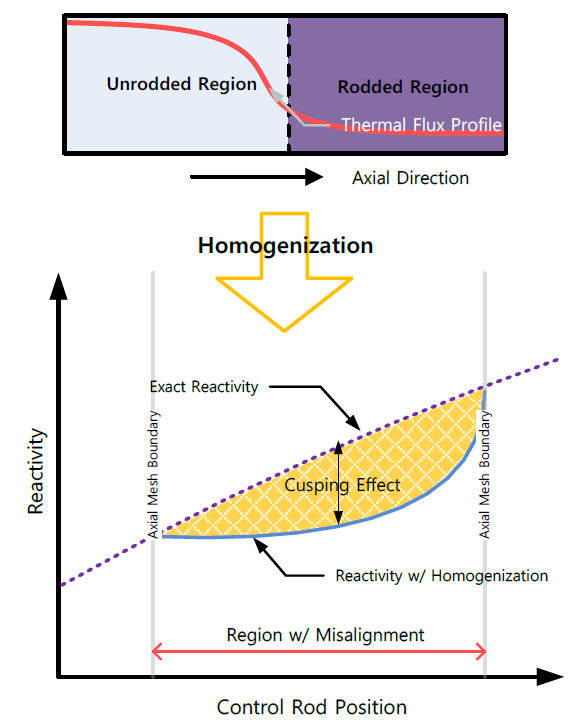
\includegraphics[width=0.4\textwidth]{cusping_effect_Joo.png}
    \caption{Illustration of Rod ``Cusping''}\label{f:cuspingEffectJoo}
\end{figure}
\todo{cite}

In some cases, this is easily handled by setting up an appropriate axial mesh which prevents the need for the homogenization, but this is not always a practical solution.  Throughout the course of an entire cycle of operation (usually about 18 months), several different control banks in the reactor may move to a variety of positions to maintain criticality in the core.  Control rods in a PWR typically have step sizes of approximately 1.5 cm, but a typical MOC plane in MPACT is about 8 cm thick in the active fuel region.  In order to prevent cusping effects for an entire cycle, the user may have to create a very detailed axial mesh to ensure that all the control rod positions used throughout the cycle align with the edge of an MOC plane.  Not only is this tedious for the user, but it also greatly increases the computational burden due to the increased number of MOC planes.  Figure \ref{f:p4cuspingEffects} shows the calculated k-eff as a function of control rod position.  The cusping effects in this figure are further complicated by a heterogeneous rod with AIC and B$_4$C poison regions and a stainless steal tip.  Thus, cusping effects occur not just at the control rod tip, but also at material interfaces throughout the rod.

\begin{figure}
    \centering
    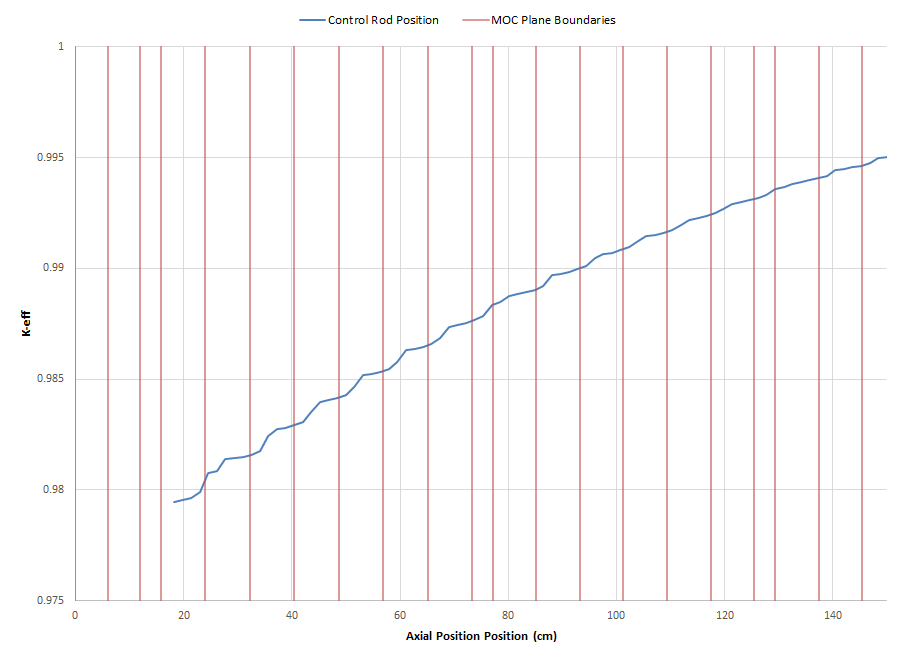
\includegraphics[width=0.8\textwidth]{p4cuspingEffects.png}
    \caption{Control Rod Cusping Effects for 3x3 Assembly}\label{f:p4cuspingEffects}
\end{figure}

\section{Traditional Solutions}

\subsection{Nodal Codes}

\todo{Legacy decusping methods}

\subsection{2D/1D Codes}\label{ss:2d1d-old-decusping-methods}

Several codes that have employed the 2D/1D method in recent years have also required rod decusping methods.  MPACT currently uses a simple polynomial correction to the volume fractions used to homogenize the control rod \cite{MC2015_VCS_Cycle_Depletion}.  To develop this method, a 3x3 assembly was set up with a control rod in the center assembly.  This problem was simulated with the rod tip at nine different positions in the plane.  These simulations were then repeated, but with the axial mesh refined so the rod tip aligned with a plane boundary.  The k-eff differences between the two sets of simulations were fitted with a sixth-order polynomial which is used in MPACT to reduce the volume fraction of the control rod by an appropriate amount to offset the cusping effects.  This process was repeated for different control rod materials such as AIC, B$_4$C, and Tungsten, since each material has unique cross-sections.  This method has the advantages of being simple to implement and requiring no increase in computational requirements.  However, the results obtained from this decusping method are tied to the control rod material and reactor model used to develop the corrections, limiting its usefulness to a small subset of reactors.

Another 2D/1D code is nTRACER, which is under active development by Seoul National University\todo{new citation}.  To address rod cusping effects in nTRACER, Jung and Joo developed a more general method than the polynomial correction method used by MPACT \cite{ICAPPcontrolRodDecuspingNTRACER}.  This method pre-generates correction factors at the start of a simulation, rather than relying on hard-coded corrections.  To do this, the assembly that will have a partially inserted control rod is identified, and a single-plane 3x3 assembly problem is set up using the partially-rodded assembly and its neighbors.  The radial and axial cusping effects are then determined separately.  First, the radial cusping effects are determined by performing 2D MOC calculations on the 3x3 sub-domain with the rod fully inserted and fully withdrawn.  This provides radial flux profiles in the rodded assembly for both rodded and unrodded regions, as well as current coupling coefficients for CMFD for the rodded and unrodded CMFD nodes.  Once this is done, the rod is simulated at positions of 25\%, 50\%, and 75\% withdrawn from the plane.  To reduce runtime, these calculations are done using only 3D sub-plane CMFD.  This generates axial flux profiles for the full MOC plane for each of the possible rod positions.  During the full-core 2D/1D calculation, these axial flux profiles are then used to generate improved homogenized cross-sections for the MOC calculation using equation.

\begin{equation}\label{e:nTRACERdecusping}
\overline{\Sigma_i} = \frac{\phi_{rad,i}^R \phi_{ax,i}^R \Sigma_i^R h^R + \phi_{rad,i}^U \phi_{ax,i}^U \Sigma_i^U h^U}{\phi_{rad,i}^R \phi_{ax,i}^R h^R + \phi_{rad,i}^U \phi_{ax,i}^U h^U}
\end{equation}

\todo{Look into other 2D/1D codes (decart)}

\section{Improved Decusping Methods}
\todo{Better Title?  Not that much ``better''}

This section discusses two new decusping treatments added to MPACT.  These methods rely on the sub-plane scheme described in section \todo{ref}.  The first method only treats the axial cusping effects, while the second method extends the first by also treating the radial decusping effects.

\subsection{Sub-plane Decusping}

In section \todo{section num}, the sub-plane scheme was introduced as a means of coarsening the 2D/1D axial mesh to improve runtime while maintaining accuracy.  However, one negative consequence of using the sub-plane scheme is that it increases the likelihood of partially inserted rods being present since there are fewer, thicker MOC planes.  To address this, two modifications were made to the sub-plane scheme to minimize cusping effects.

The first modification that was made was to modify the cross-sections used for the sub-plane CMFD and axial SP$_3$ calculations.  In the most basic form of the sub-plane scheme, the same cross-sections and radial coupling coefficients are used for all sub-planes in each MOC plane.  To use sub-plane as a decusping method, the requirement for constant cross-sections was removed.  Thus, when equation \ref{e:CMFDhomogTerms} is applied, explicit rodded or unrodded cross-sections are used for the cross-section homogenization in each sub-plane, rather than a single homogenized cross-section being using in all sub-planes.  This allows the CMFD and axial solvers to capture the sharp flux gradients that occur around the edge of the control rods.

In order to improve the MOC calculations as well, the CMFD flux projection described in equation \ref{e:CMFDscaling} is extended to also include a cross-section projection for the partially rodded pin cells.  This is done using equation \ref{e:nTRACERdecusping} with $\phi_{rad,i}^R = \phi_{rad,i}^U$.  This allows the 2D MOC calculations to also capture some of the axial effects of the partially inserted rod.

\subsection{Auxiliary 1D Collision Probabilities}

While the sub-plane decusping method is better than none, it captures only the axial effects of the partially inserted rod.  To also capture the radial effects, an additional radial calculation is needed to obtain radial flux profiles for the rodded and un-rodded regions.  In MPACT, this is done using a 1D Collision Probabilities (CP) solver.

After the CMFD homogenization, but prior to the calculation itself, a 1D CP kernel is solved for the rodded and un-rodded regions to obtain a radial flux profile.  These profiles are normalized so that the volume-average of each profile is exactly unity.  These profiles are then used with the sub-plane CMFD flux and material cross-sections to calculate improved homogenized cross-sections, as shown in equation \ref{e:CPMxs}.  Homogenizing the cross-sections in this way allows CMFD to capture both axial and radial effects of the partially inserted rod with negligible increase in computational expense.  This process is illustrated in figure \ref{f:CPdecusp}.

\begin{equation}\label{e:CPMxs}
\Sigma_{g,i}=\frac{1}{\phi_{g,i}V_i}\sum_{r=1}^{N_{rings}} \Sigma_{g,r} \phi_{CMFD,g,i} \phi_{CP,g,r} V_r
\end{equation}

\begin{figure}
  \centering
  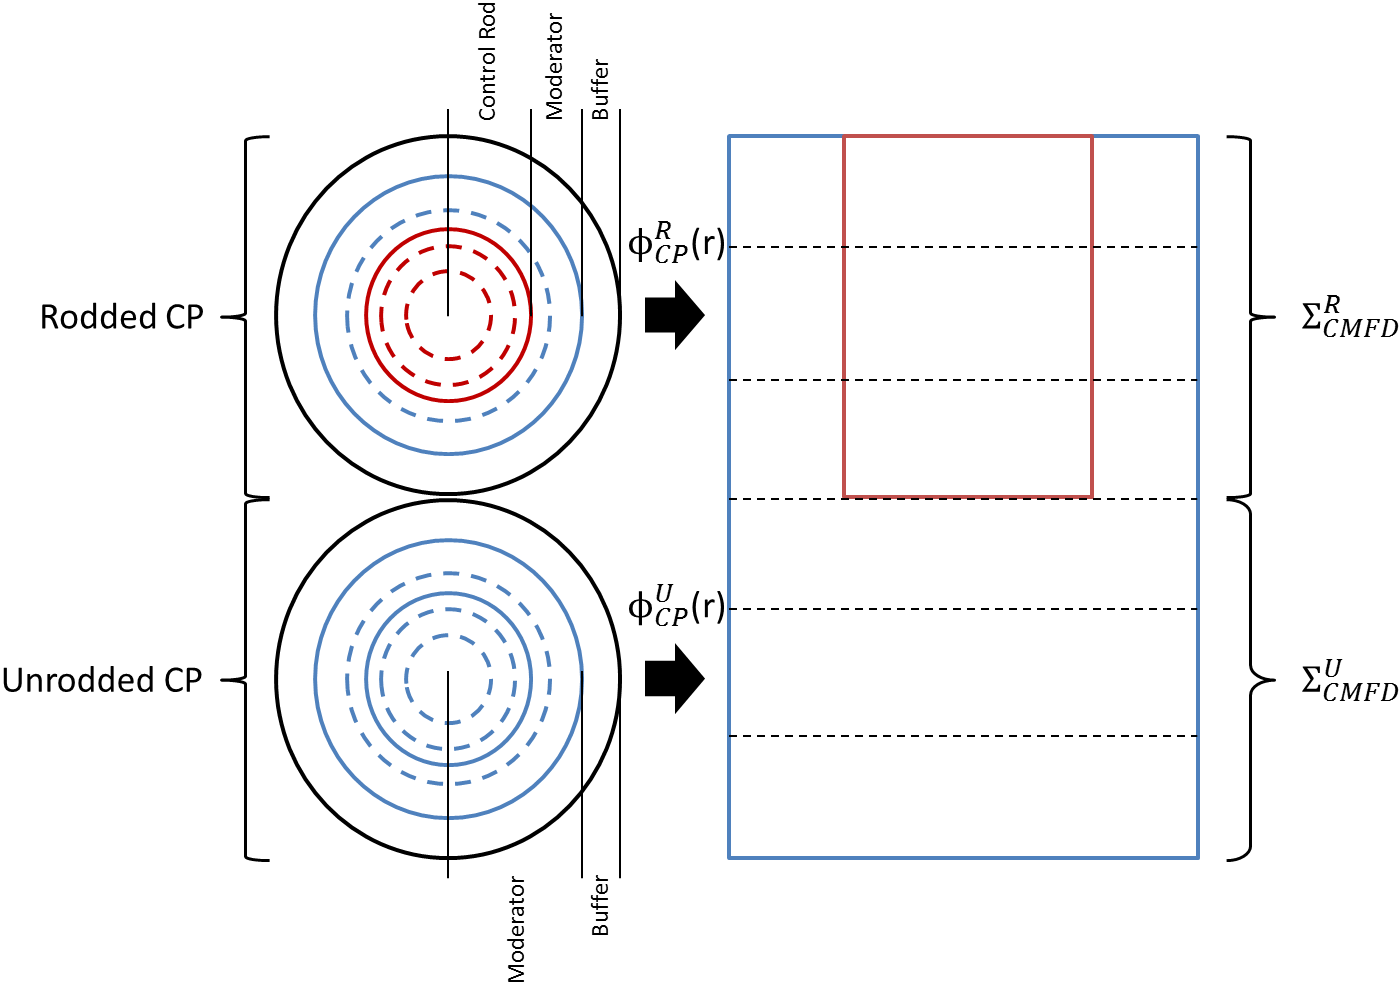
\includegraphics[width=\textwidth]{CPdecusp.png}
  \caption[Collision Probabilities Decusping]{Illustration of 1D Collision Probabilities rod decusping method}\label{f:CPdecusp}
\end{figure}

After the CMFD calculation, the MOC cross-sections must be modified as with the sub-plane decusping.  This is done using by using equation \ref{e:nTRACERdecusping} directly, where the radial flux terms are the projected MOC fluxes and the axial flux terms are the results of the sub-plane CMFD calculation that used the CP-homogenized cross-sections.  The projection of the CMFD flux to the MOC mesh is unchanged from the standard sub-plane scheme.  The CMFD calculation flow when using 1D CP is shown in figure \ref{f:1dcpm-flowchart}

\begin{figure}
  \centering
  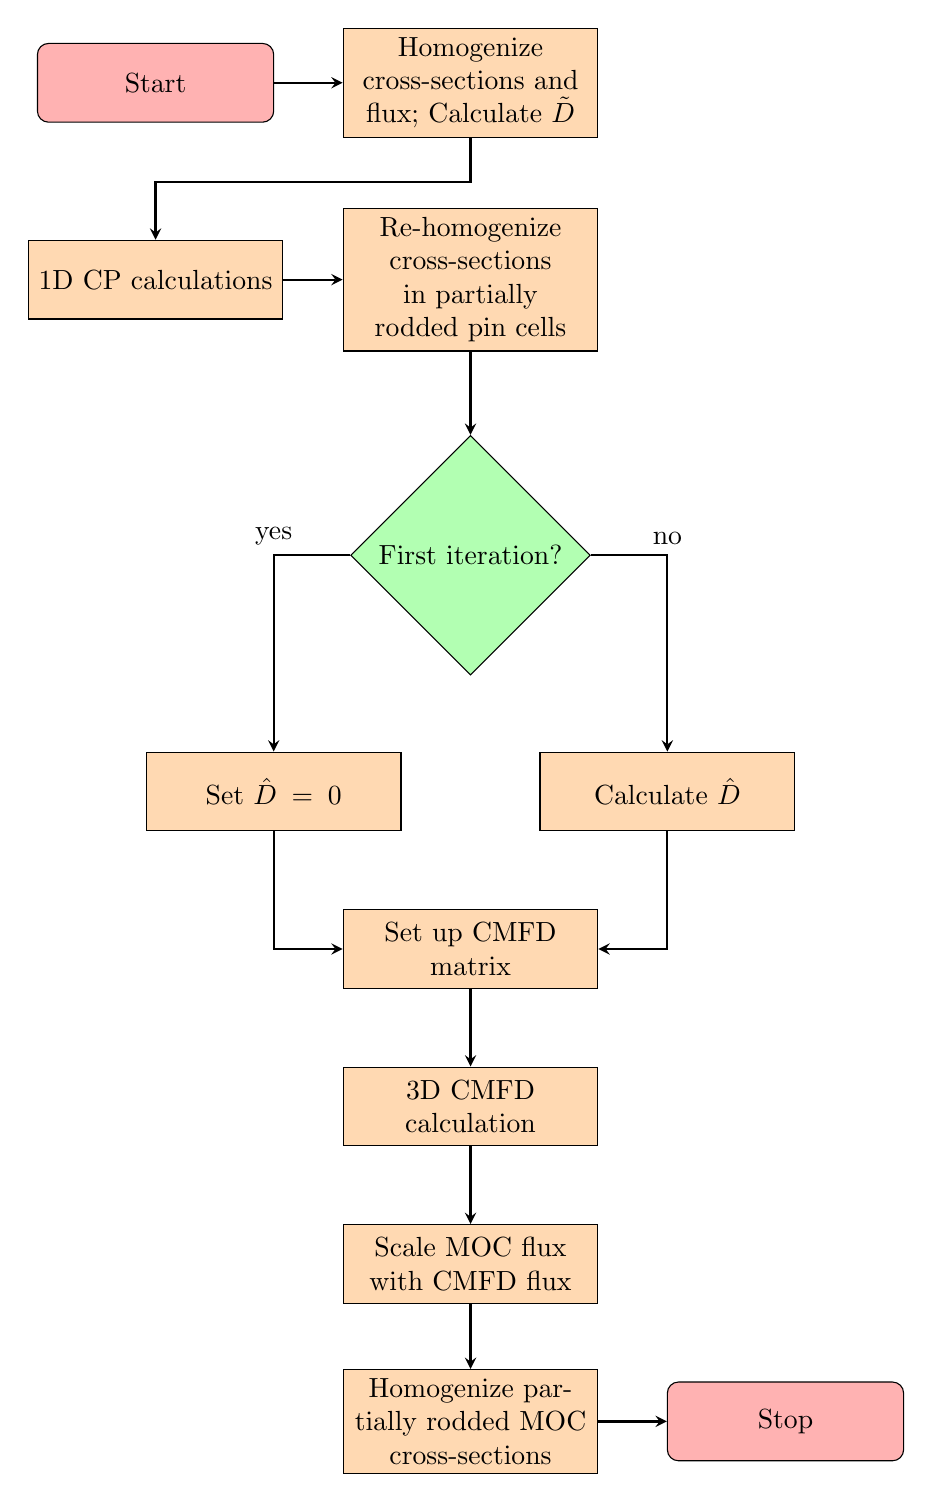
\begin{tikzpicture}[node distance=2cm]

% Start
\node (start) [startstop] {Start};

% CMFD
\node (homog) [process, right of=start, xshift=2.0cm] {Homogenize cross-sections and flux; Calculate $\tilde{D}$};
\node (1dcpm) [process, below of=start, yshift=-0.5cm] {1D CP calculations};
\node (homogCP) [process, right of=1dcpm, xshift=2.0cm] {Re-homogenize cross-sections in partially rodded pin cells};
\node (iterCheck) [decision, below of=homogCP, yshift=-1.5cm] {First iteration?};
\node (firstIter) [process, below of=iterCheck, xshift=-2.5cm, yshift=-1.0cm] {Set $\hat{D}=0$};
\node (laterIter) [process, below of=iterCheck, xshift=2.5cm, yshift=-1.0cm] {Calculate $\hat{D}$};
\node (matrix) [process, below of=firstIter, xshift=2.5cm] {Set up CMFD matrix};
\node (3DCMFD) [process, below of=matrix] {3D CMFD calculation};
\node (proj) [process, below of=3DCMFD] {Scale MOC flux with CMFD flux};
\node (projCP) [process, below of=proj] {Homogenize partially rodded MOC cross-sections};

% Stop
\node (stop) [startstop, right of=projCP, xshift=2.0cm] {Stop};

% Basic Arrows
\draw [arrow] (start) -- (homog);
\draw [arrow] (1dcpm) -- (homogCP);
\draw [arrow] (homogCP) -- (iterCheck);
\draw [arrow] (matrix) -- (3DCMFD);
\draw [arrow] (3DCMFD) -- (proj);
\draw [arrow] (proj) -- (projCP);
\draw [arrow] (projCP) -- (stop);

% Fancy Arrows
\draw [arrow] (homog) |- ([yshift=-0.75cm]start.south) -| (1dcpm);
\draw [arrow] (iterCheck) -| node[anchor=south] {yes} (firstIter);
\draw [arrow] (iterCheck) -| node[anchor=south] {no} (laterIter);
\draw [arrow] (firstIter) |- (matrix);
\draw [arrow] (laterIter) |- (matrix);

\end{tikzpicture}
  \caption[Stuff]{Calculation flow for CMFD calculation in MPACT with 1D CP decusping treatment}\label{f:1dcpm-flowchart}
\end{figure}

\chapter{Results}
\begin{frame}[t]{VERA Problem 4}
    
    
    
\end{frame}

%%%%%%%%%%%%%%%%%%%%%%%%%%%%%%%%%%%%%%%%%%%%%%%%%%%%%%%%%%%%%%%%%%%%%%%%%%%%%%%%%

\begin{frame}[t]{Problem 4 Results}
    
    
    
\end{frame}

%%%%%%%%%%%%%%%%%%%%%%%%%%%%%%%%%%%%%%%%%%%%%%%%%%%%%%%%%%%%%%%%%%%%%%%%%%%%%%%%%

\begin{frame}[t]{VERA Problem 5}
    
    
    
\end{frame}

%%%%%%%%%%%%%%%%%%%%%%%%%%%%%%%%%%%%%%%%%%%%%%%%%%%%%%%%%%%%%%%%%%%%%%%%%%%%%%%%%

\begin{frame}[t]{Problem 5 Results}
    
    
    
\end{frame}
 
\chapter{Conclusions}
\input{06-conclusions.tex}

% bibliography
\renewcommand{\bibname}{References}
\addcontentsline{toc}{chapter}{References}
% TODO: Add bibliography

%appendices
\begin{appendices}



\end{appendices}

\end{document}